\documentclass{sig-alternate}

\usepackage{graphicx}


\usepackage{url}
\usepackage{hyperref}
\hypersetup{breaklinks}

\begin{document}
\title{Adaptive and Heterogeneous Hadoop MapReduce}
\author{Aaron Burkhart, Ross Nordstrom\\
        University of Colorado - Colorado Springs\\
        1420 Austin Bluffs Pkwy,\\
        Colorado Springs, CO 80918\\
        \texttt{\{aburkhar,rnordstr\}@uccs.edu}
       }
\date{April 2014}

\maketitle

\begin{abstract}
Hadoop is a commonly used Apache implementation of MapReduce, a technique for
parallel processing in distributed systems. One weakness of Hadoop is it does
not compute input splits or assign tasks based on the computers' computational capabilities.
This causes an execution time skew between nodes, leaving high performing nodes waiting
for low performing nodes to finish. This skew can also be caused by interference from
third party VMs running on the same hardware as nodes in the Hadoop cluster. By scaling
how much work is sent to a given computer based on its capabilities, we can
redce the difference in task completion time across the system, and thus improve
the overall performance of Hadoop. We call such a system -- with computers of
varying capabilities -- a heterogeneous environment. This research aims to develop
a task scheduling and assignment algorithm for Hadoop MapReduce that is sensitive
to both the hardware configurations of the nodes in the cluster and interference
from other non-cluster nodes running on the same hardware as cluster node.
\end{abstract}

\category{C.2.4}{Performance}{Cloud computing}
\terms{Performance, Design}
\keywords{Hadoop, MapReduce, Heterogeneous, Configuration, Cloud}

\section{Introduction}
Hadoop MapReduce is well-liked for its ability to dispatch tasks across workers
in a datacenter. Hypothetically, if the work is split up into equal parts and dispatched
efficiently across similar nodes, the system will work well. In reality, datacenters today are being
updated continuously with new hardware, while old hardware lingers in the datacenter.
Some customers are willing to pay more for high performing nodes, while others prioritize cost over
performance. This diversity in customer needs contributes to diversity in datacenter hardware.
Additionally, most consumers of datacenters are not the owners. Take Amazon EC2
or Windows Azure, for example. Companies maintain datacenters and sell access to
it as a service.

Because modern datacenters are so frequently consumed as a service, the consumer
has little control over what hardware to which they will have access. Even if the
consumer had full control over which hardware they accessed, it is costly and
inefficient to maintain a datacenter full of machines with identical hardware.
Additionally, creating an algorithm to deploy a given MapReduce job across only
identical machines would be difficult.

Another issue with modern datacenters, is that the hardware is shared between users.
The user deploying a Hadoop cluster usually won't have control over which physical
machines their VMs will be deployed to and there may very well be other users with
VMs sharing and competing for physical hardware resources. This can cause performance
degradation for some of the nodes in your cluster, further imbalancing execution time.
This is true for both homogeneous and heterogeneous clusters.

Rather than fight the structure of datacenters, adapting Hadoop to the environment
in which it is deployed would allow for optimal MapReduce performance in arbitrary
environments. This is especially important when deploying Hadoop using an IaaS
(infrastructure as a service).

Our research aims to modify Hadoop v1.2.1 to adaptively vary the sizes of the input
splits and dispatch MapReduce tasks based on both the workers' computational power
and scheduling status. In this paper, we discuss the existing implementation of Hadoop
and elaborate the issues it has when executing on heterogeneous environments. We then
describe our solution in more detail and evaluate our resulting implementation. Finally
we suggest directions for future work and improvements to our progress.

\section{Motivation}
\label{section:motivation}
Hadoop MapReduce is an easy-to-use implementation of distributed, parallel data 
processing. It has a history of making it easy for data scientists and industry 
developers to implement parallel computing in the cloud, but for the serious 
user of Hadoop, there is room for improvement. Hadoop does most things well, 
but we propose a modification to it that would improve its performance for all 
users.

\subsection{Homogeneous Task Assignment}
Hadoop MapReduce assumes homogeneous hardware configurations for the nodes in 
its cluster when it schedules and assigns tasks to them. If the nodes in the 
cluster in fact have heterogeneous hardware configurations then the execution 
and completion times of these tasks could vary in unanticipated ways. 
Additionally, interference from non-cluster nodes running on the same hardware 
could change performance as well. These two problems can cause inefficient 
resource usage and degraded performance. 

\subsection{Modifying Hadoop}
A new scheduling and assignment algorithm is needed that is capable of 
identifying the hardware configurations of the nodes in its cluster and 
scheduling tasks on them accordingly. This algorithm should also be sensitive 
to interference from other non-cluster nodes and adapt. The hardware 
configurations of the cluster nodes can be set ahead of time, however, 
interference from non-cluster nodes cannot be anticipated. This algorithm 
should be able to detect interference and dynamically change the task settings 
accordingly.

The existing Hadoop task scheduler/assignment module will need to be identified 
in the source code for Hadoop 1.2.1. It will then need to be either modified or 
replaced to meet the requirements proposed in this document. A server cluster 
with heterogeneous hardware configurations will be created and used to test the 
performance of the system. Both the modified and unmodified code will be built 
and deployed on this cluster. Both will run the same MapReduce job and the 
performance of each will be compared.

\section{Related Work}
\label{section:relatedwork}
Hadoop MapReduce is a popular subject of research. The primary focus of the research
is on performance improvement. While the proposals other authors have made vary in
approach and effectiveness, we have not yet found an approach similar to the one
we propose.

Here, we list a few of the other approaches to performance improvement that we have found:
\begin{description}
  \item{Levitated Merge:} Improves the performance of MapReduce by focusing on network latency between workers \cite{LevitatedMerge}.
  \item{SHadoop:} Improves MapReduce performance by optimizing the job and task execution \cite{SHadoop}.
  \item{HJ-Hadoop:} Improves MapReduce performance by optimizing for multi-core machines \cite{HJHadoop}.
  \item{I/O-Intensive Hadoop:} Improves MapReduce performance by using dynamic processing slots for I/O instensive jobs \cite{IOIntensiveHadoop}.
  \item{Hybrid MapReduce:} Improves MapReduce performance by using a combination of virtual and native environments \cite{HybridMR}.
\end{description}

\section{Proposed Design}
\label{section:propeseddesign}

Before doing any implementation, we conducted some investigation into how Hadoop works, 
specifically how it assigns tasks initially and how they are reassigned during runtime.
These are important attributes to understand, because they contribute to uneven effective
workloads in a heterogeneous environment; that is, if two machines are assigned equal-sized
tasks, but one machine is twice as powerful as the other, it was effectively given half as
much work since it will complete it twice as fast as the other machine.

\subsection{Hadoop MapReduce Task Assignment}
In standard Hadoop MapReduce, the Mapper divides up and distributes tasks to the workers.
Understanding this implementation is key to our research so that we can scale task sizes
to the computational capabilities of each MapReduce node. In Hadoop, a \texttt{JobConf}
object defines the configuration for each Mapper. By customizing this object per node,
we should be able to scale how much work a given node is given based on its capabilities.

A naive approach to scaling node task assignment would be to perform some basic performance
diagnostics during the task setup phase, and apply a simple weight coefficient to how much
work it should receive.

\subsection{Hadoop MapReduce Reduces}
In addition to hetergeneous machines, datacenters can also exhibit temporal heterogeneity.
VM performance depends on the behavior of other VMs on the same machine at any given time.
This means a VM on a machine with other, inactive VMs will initially be very performant;
but once the other VMs begin doing work the VM will experience performance degradation.
The variability of a VM's performance also depends on the abstraction layer between the VMs
and the physical hardware.


\section{Implementation}
\label{section:implementation}
Using Hadoop v1.2.1, we were able to build and run a wordcount job
on both a single-node setup and a distributed two-node setup. Once
we had achieved this, we began instrumenting the code with extra,
custom logging to better understand how Hadoop works. Using the
logging and growing understanding of the Hadoop code base, we were
able to identify a couple key code insertion/modification points.

\subsection{Modifying Split Sizes}
One of the fundamental tasks we set out to achieve was to modify the
sizes of input splits. We found that the \texttt{InputSplit.getSplits()}
method, defined in \texttt{FileInputFormat.java} offered the cleanest
point for us to modify the splits. We opted for a contrived proof of
concept implementation, where we treated the job as static (by running
the same job repeatedly on the same machines) and forcing half of the
splits to be large. Our modification aims to be unobtrusive to Hadoop's
normal split algorithms by simply using a \texttt{minSize} to force larger
splits to occur. The code to do so is shown in \ref{fig:getSplitsCode}.

\begin{figure}[ht!]
\centering
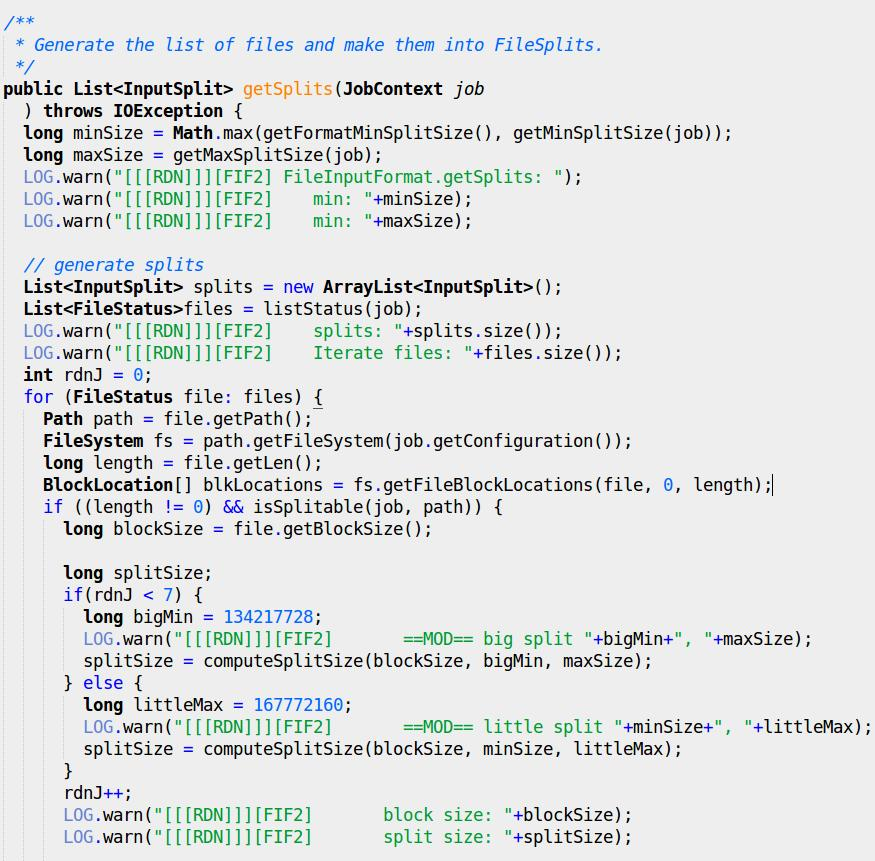
\includegraphics[width=90mm]{getSplitsCode.jpg}
\caption{Code coercing modified split sizes}
\label{fig:getSplitsCode}
\end{figure}

We then used log statements to confirm the splits were modified successfully.
An example of these log statements is shown in \ref{fig:getSplitsLog}.

\begin{figure}[ht!]
\centering
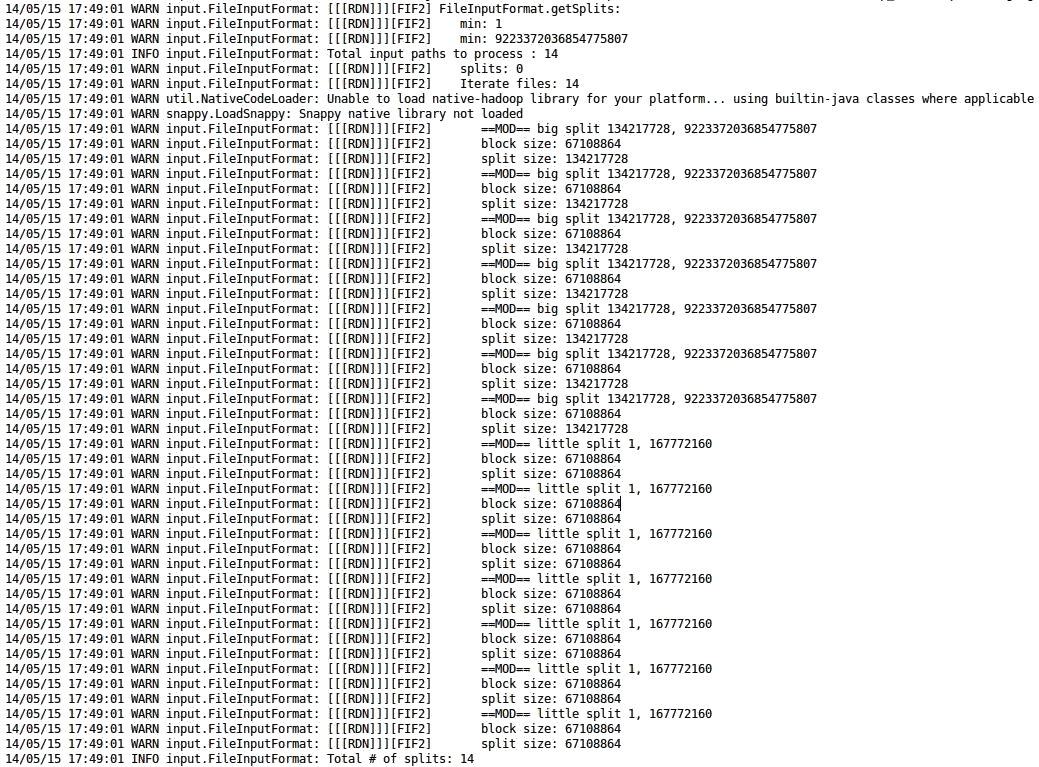
\includegraphics[width=90mm]{getSplitsLog.jpg}
\caption{Logs showing modified split sizes in a wordcount job}
\label{fig:getSplitsLog}
\end{figure}

\subsection{Classifying Host Capabilities}
Simply creating different size input splits is not sufficient for increasing
performance without associating which node or classification of node should
get which size split. There are several ways in which this can be done.
The simplest way to tie performance information to nodes in the Hadoop
environment would be to create a file in the \texttt{conf/} directory with
this information, and modifying the
\texttt{JobConf} class to parse in any new properties we define. A rudimentary
method would be to define two or more static input split sizes and two or more
classifications of nodes, identifying which nodes belong to which category.
We would then
use this configuration to determine how many and of what size splits to make
in \texttt{getSplits}, and then which nodes should get which sized splits
in the \texttt{TaskScheduler}. The \texttt{TaskScheduler} uses the
\texttt{TaskTrackerStatus} to get information about the node it is currently
assigning tasks to. This class could be modified to contain the classification
information about that node and then it could determine which input split size
to give it. A more dynamic solution would be to have each node report current
performance metrics in its \texttt{heartbeat} to the JobTracker. This metric
would then determine what input split size to give it. This method would also be
somewhat sensitive to degraded performance on that node caused by interference
from third party VMs running on the same hardware.

\section{Future Work}
\label{section:futurework}

There is some remaining work to be done to fully qualify our Adaptive Hadoop idea. Additionally, 
assuming our idea holds, there are a number of potential extensions of our work. In section we
describe both sets of future work.

\subsection{Immediate Work}

\subsection{Extension Work}
Another approach to balancing the execution of MapTasks would be to calculate input splits
dynamically instead of creating them all ahead of time. When a slot is open on a \texttt{TaskTracker}, it would
be assigned a task with an input split that gets created with a size appropriate for the current circumstances
and the processing capabilities of the node it will be executed on.

\section{Conclusion}
\label{section:conclusion}
Our project was a difficult one, simply because building and deploying
Hadoop MapReduce is not trivial. Setting up our environment took up a
significant amount of our time. A benefit of this difficulty is the
extra work we did up front helped us gain a better understanding of
Hadoop.

The work we achieved was, we believe, a solid step towards proving our
hypothesis that modifying input split sizes based on the capabilities
of nodes in the Hadoop environment can optimize performance in heterogeneous
environments.

Our work left off on the cusp of vetting the idea. The major remaining
pieces to be done (described in \ref{section:futurework}) could be done without
significantly more work, and would be enough to validate the idea with
some benchmarking.

\bibliography{citations}{}
\bibliographystyle{plain}

\end{document}

